\documentclass[svgnames,11pt]{beamer}
\input{/home/tof/Documents/Cozy/latex-include/preambule_commun.tex}
\input{/home/tof/Documents/Cozy/latex-include/preambule_beamer.tex}
%\usepackage{pgfpages} \setbeameroption{show notes on second screen=left}
\author[]{Christophe Viroulaud}
\title{TP flocon de von Koch}
\date{}
%\logo{}
\institute{Terminale - NSI}

\begin{document}
\begin{frame}
\titlepage
\end{frame}
\begin{frame}
    \frametitle{}

    Le flocon de von Koch est l'une des premières courbes fractales à avoir été décrites (bien avant l'invention du terme \emph{fractal}). Elle a été inventée en 1904 par le mathématicien suédois Helge von Koch.
    \begin{center}
    \centering
    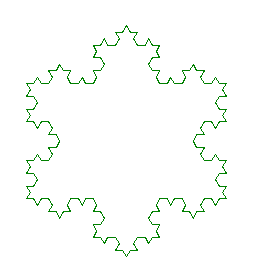
\includegraphics[width=5cm]{ressources/flocon.png}
    \captionof{figure}{flocon de von Koch}
    \label{IMG}
    \end{center}

\end{frame}
\begin{frame}
    \frametitle{}

    \begin{center}
        \begin{framed}L'objectif de cette séance est de créer un programme récursif permettant de dessiner un flocon de von Koch
        \end{framed}
    \end{center}

\end{frame}
\section{Bibliothèque \textbf{\texttt{turtle}}: rappels}
\begin{frame}
    \frametitle{Bibliothèque \textbf{\texttt{turtle}}: rappels}

    La bibliothèque \textbf{\texttt{turtle}} permet de dessiner des figures géométriques simplement. La documentation se trouve ici:
\begin{center}
\url{https://docs.python.org/fr/3.8/library/turtle.html}
\end{center}
\end{frame}
\begin{frame}[fragile]
    \frametitle{}

    \begin{activite}
 Créer un fichier \textbf{\texttt{spirale.py}}, importer la bibliothèque \textbf{\texttt{turtle}} et l'initialiser avec les paramètres suivants:
\begin{center}
\begin{lstlisting}[language=Python , basicstyle=\ttfamily\small, xleftmargin=2em, xrightmargin=2em]
colormode(255)
speed(5)
hideturtle()
\end{lstlisting}
\end{center}

    \end{activite}
\begin{center}
\centering
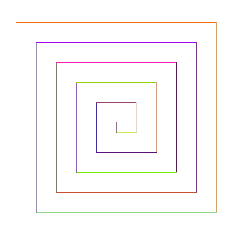
\includegraphics[width=3cm]{ressources/spirale.png}
\captionof{figure}{Figure à obtenir à la fin de l'activité}
\end{center}
\end{frame}
\begin{frame}
    \frametitle{}
Pour dessiner la figure, le programme respecte l'algorithme:
\begin{itemize}
    \item choisir une couleur,
    \item tracer un trait de dimension \textbf{\texttt{dim}},
    \item tourner de 90°,
    \item répéter l'opération en diminuant la dimension de 10.
\end{itemize}
    \begin{activite}
    \begin{enumerate}
        \item Écrire la fonction \textbf{\texttt{creer\_couleur() $\rightarrow$ tuple}} qui renvoie un tuple (r, g, b) de trois entiers aléatoires compris entre 0 et 255.
        \item Écrire la fonction récursive \textbf{\texttt{dessiner(dim: int) $\rightarrow$ None}} qui respecte l'algorithme.
        \item Exécuter la fonction avec une dimension de 200.
    \end{enumerate}
    \end{activite}

\end{frame}
\begin{frame}
    \frametitle{Avant de regarder la correction}
\begin{center}
    \centering
    \includegraphics[width=3cm]{/home/tof/Documents/Cozy/latex-include/stop.png}
    \end{center}
{\Large
    \begin{itemize}
        \item Prendre le temps de réfléchir,
        \item Analyser les messages d'erreur,
        \item Demander au professeur.
    \end{itemize}
}
\end{frame}
\begin{frame}[fragile]
    \frametitle{Correction}

    \begin{center}
    \begin{lstlisting}[language=Python , basicstyle=\ttfamily\small, xleftmargin=2em, xrightmargin=1em]
def creer_couleur() -> tuple:
    """
    renvoie une couleur (r, g, b)
    """
    return (randint(0, 255) for _ in range(3))
\end{lstlisting}
    \captionof{code}{Choix de la couleur}
    \label{CODE}
    \end{center}

\end{frame}
\begin{frame}[fragile]
    \frametitle{Correction}

    \begin{center}
    \begin{lstlisting}[language=Python , basicstyle=\ttfamily\small, xleftmargin=2em, xrightmargin=2em]
def dessiner(dim: int) -> None:
    """
    dessine une spirale carrée
    """
    if dim >= 0:
        pencolor(creer_couleur())
        forward(dim)
        right(90)
        dessiner(dim-10)  

dessiner(200)
\end{lstlisting}
    \captionof{code}{Dessiner}
    \label{CODE}
    \end{center}

\end{frame}
\section{Flocon de von Koch}
\subsection{Principe}       
\begin{frame}
    \frametitle{Principe}

    On peut créer le flocon à partir d'un segment de droite, en le modifiant récursivement selon la précision désirée:
    \begin{itemize}
    \item Diviser le segment en trois segments de longueurs égales.
    \item Tourner de 60°.
    \item Recommencer pour chaque segment obtenu.
    \end{itemize}
    \begin{center}
        \begin{tabular}{cc}
            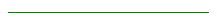
\includegraphics[width=4cm]{ressources/koch0.png}
            &
            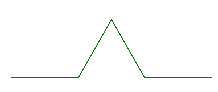
\includegraphics[width=4cm]{ressources/koch1.png}\\
            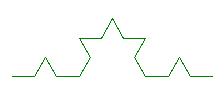
\includegraphics[width=4cm]{ressources/koch2.png}
            &
            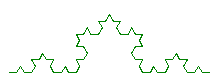
\includegraphics[width=4cm]{ressources/koch3.png}\\
        \end{tabular}
        \captionof{figure}{Étapes de construction}
        \label{etapes}
    \end{center}

\end{frame}
\subsection{Construction récursive}
\begin{frame}
    \frametitle{Construction récursive}
\begin{activite}
\begin{enumerate}
    \item Observer la figure \ref{etapes} pour déterminer les étapes récursives.
    \item Quelle est l'étape limite (qui stoppe les appels récursif)?
\end{enumerate}
\end{activite}
    

\end{frame}
\begin{frame}
    \frametitle{Avant de regarder la correction}
\begin{center}
    \centering
    \includegraphics[width=3cm]{/home/tof/Documents/Cozy/latex-include/stop.png}
    \end{center}
{\Large
    \begin{itemize}
        \item Prendre le temps de réfléchir,
        \item Analyser les messages d'erreur,
        \item Demander au professeur.
    \end{itemize}
}
\end{frame}
\begin{frame}
    \frametitle{Correction}

Chaque trait est partagé en 3 morceaux. En prenant en compte les rotations on obtient 4 traits. Au lieu de tracer un trait, l'étape récursive consiste à partager à nouveau ce trait.\\L'étape finale consiste à tracer effectivement un trait. Elle est atteinte quand on arrive à la précision désirée.

\end{frame}
\begin{frame}
    \frametitle{}

    \begin{activite}
    Écrire la fonction \textbf{\texttt{courbe\_koch(precision: int, mesure: int) $\rightarrow$ None}}
    qui construit un côté du flocon (figure \ref{etapes}).
\end{activite} 

\end{frame}
\begin{frame}
    \frametitle{Avant de regarder la correction}
\begin{center}
    \centering
    \includegraphics[width=3cm]{/home/tof/Documents/Cozy/latex-include/stop.png}
    \end{center}
{\Large
    \begin{itemize}
        \item Prendre le temps de réfléchir,
        \item Analyser les messages d'erreur,
        \item Demander au professeur.
    \end{itemize}
}
\end{frame}
\begin{frame}[fragile]
    \frametitle{Correction}

\begin{center}
\begin{lstlisting}[language=Python , basicstyle=\ttfamily\small, xleftmargin=1em, xrightmargin=1em]
def courbe_koch(precision: int, mesure: int) -> None:
    if precision == 0:
        forward(mesure)
    else:
        courbe_koch(precision-1, mesure//3)
        left(60)
        courbe_koch(precision-1, mesure//3)
        right(120)
        courbe_koch(precision-1, mesure//3)
        left(60)
        courbe_koch(precision-1, mesure//3)
\end{lstlisting}
\captionof{code}{Tracer une branche}
\label{CODE}
\end{center}

\end{frame}
\subsection{Construction du flocon}
\begin{frame}
    \frametitle{Construction du flocon}

    \begin{activite}
    \begin{enumerate}
        \item Écrire la fonction \textbf{\texttt{flocon(precision: int, mesure: int) $\rightarrow$ None}} qui utilise la fonction \textbf{\texttt{courbe\_koch}} pour tracer le flocon.
        \item Tester la fonction pour plusieurs précisions. Attention le temps de tracé peut être très long pour des valeurs supérieures à 5.
        \item \textbf{Pour les plus avancés:}
        \begin{itemize}
            \item Tracer chaque trait d'une couleur différente.
            \item Construire un flocon avec la courbe suivante:
            \begin{center}
            \centering
            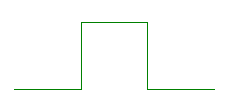
\includegraphics[width=4cm]{ressources/vonkochcarre.png}
            \end{center}
        \end{itemize}
    \end{enumerate}
    \end{activite}

\end{frame}
\begin{frame}
    \frametitle{Avant de regarder la correction}
\begin{center}
    \centering
    \includegraphics[width=3cm]{/home/tof/Documents/Cozy/latex-include/stop.png}
    \end{center}
{\Large
    \begin{itemize}
        \item Prendre le temps de réfléchir,
        \item Analyser les messages d'erreur,
        \item Demander au professeur.
    \end{itemize}
}
\end{frame}
\begin{frame}[fragile]
    \frametitle{Correction}

    \begin{center}
    \begin{lstlisting}[language=Python , basicstyle=\ttfamily\small, xleftmargin=1em, xrightmargin=1em]
def flocon(precision: int, mesure: int) -> None:
    for _ in range(3):
        courbe_koch(precision, mesure)
        right(120)


flocon(3, 500)
\end{lstlisting}
    \captionof{code}{Tracé du flocon}
    \label{CODE}
    \end{center}

\end{frame}
\begin{frame}[fragile]
    \frametitle{Correction}

    \begin{center}
    \begin{lstlisting}[language=Python , basicstyle=\ttfamily\small, xleftmargin=1em, xrightmargin=1em]
def courbe_koch_carre(precision: int, mesure: int) -> None:
    if precision == 0:
        forward(mesure)
    else:
        courbe_koch_carre(precision-1, mesure//3)
        left(90)
        courbe_koch_carre(precision-1, mesure//3)
        right(90)
        courbe_koch_carre(precision-1, mesure//3)
        right(90)
        courbe_koch_carre(precision-1, mesure//3)
        left(90)
        courbe_koch_carre(precision-1, mesure//3)
\end{lstlisting}
    \captionof{code}{von Koch quadratique}
    \label{CODE}
    \end{center}

\end{frame}
\begin{frame}[fragile]
    \frametitle{Correction}

    \begin{center}
    \begin{lstlisting}[language=Python , basicstyle=\ttfamily\small, xleftmargin=1em, xrightmargin=1em]
def flocon_carre(precision: int, mesure: int) -> None:
    for _ in range(4):
        courbe_koch_carre(precision, mesure)
        right(90)
\end{lstlisting}
    \end{center}
\begin{center}
\centering
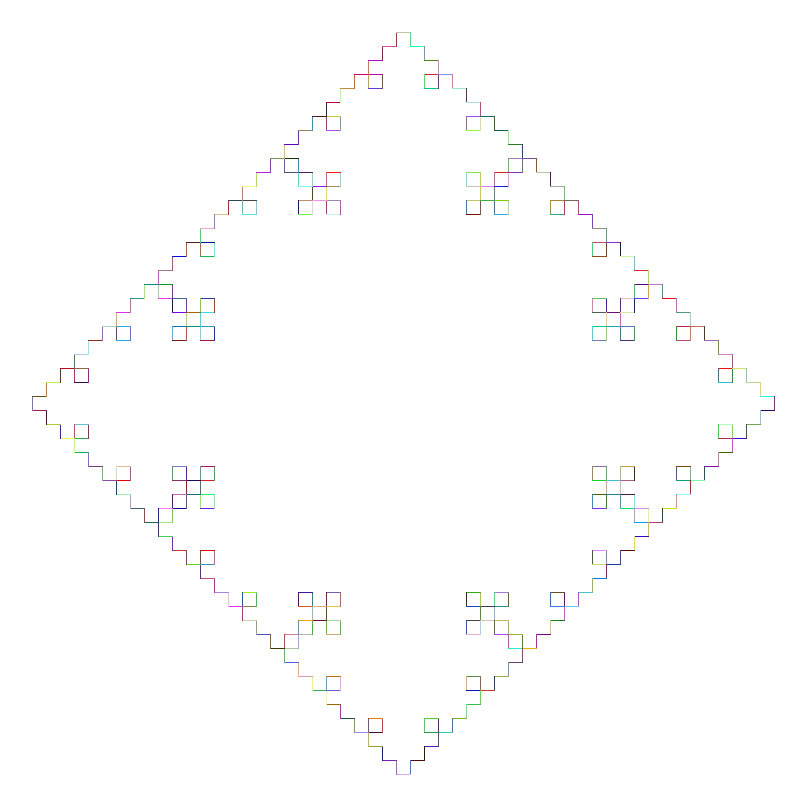
\includegraphics[width=5cm]{ressources/quadratique.png}
\end{center}
\end{frame}
\end{document}